\documentclass[11pt]{article}

% Language setting
% Replace `english' with e.g. `spanish' to change the document language
\usepackage[english]{babel}

% Set page size and margins
% Replace `letterpaper' with `a4paper' for UK/EU standard size
\usepackage[letterpaper,top=2cm,bottom=2cm,left=3cm,right=3cm,marginparwidth=1.75cm]{geometry}

% Change the space inserted between paragraphs and remove indent
\usepackage{parskip}

% Useful packages
\usepackage{amsmath}
\usepackage{mathtools}
\usepackage{graphicx}
\usepackage{amssymb}
\usepackage{amsfonts}
\usepackage{physics}
\usepackage{gensymb}
\usepackage{mathrsfs}
\usepackage{multirow}
\usepackage[colorlinks=true, allcolors=blue]{hyperref}

% Highlight parts of matrices   `'
\usepackage{tikz}
\usetikzlibrary{fit}
\tikzset{
  highlight/.style={rectangle, rounded corners, fill=red!15, draw, fill opacity=0.4, thick, inner xsep=4pt, inner ysep=0pt}
}

\newcommand{\tikzmark}[2]{\tikz[overlay,remember picture,
  baseline=(#1.base)] \node (#1) {#2};}

\newcommand{\Highlight}[1][submatrix]{
    \tikz[overlay, remember picture]{
        \node[highlight, fit=(left.north west) (right.south east)] (#1) {};
    }
}

% Set maximum number of columns in matrices
\setcounter{MaxMatrixCols}{13}

% Make quotes
\usepackage{csquotes}

% Bibliography management
\usepackage{biblatex}
\addbibresource{sample.bib}

% Specify path to images folder. The path is relative to the current working directory
\graphicspath{{./images/}}

\DeclareMathOperator{\spn}{span}
\DeclareMathOperator{\diag}{diag}
\DeclareMathOperator{\diff}{d}
\DeclareMathOperator{\diffx}{dx}

\title{Scientific Project}
\author{Fernando Muñoz Martínez}

\begin{document}

% Este código contiene el formato de la portada.
\begin{titlepage}
 
\thispagestyle{empty}

    \begin{center}
        \mbox{}\vfill
        \LARGE
        \textbf{Scientific Project} 
	
        \vspace{1 cm}
        \large
        Fernando Muñoz Martínez
        
        \vspace{1 cm}	
        \large
        Supervisor: Prof. Dr. Stefan Teufel \\
        Mathematics Department \\
        University of Tübingen

        \vspace{1 cm}
        \large
        Summer Semester 2026
    \end{center}

    \vspace{10 cm}
    \large
        
\end{titlepage}

\newpage

\tableofcontents

\newpage

\section{Introduction}

\subsection{Research Motivation}

Spectral analysis has proven to be a powerful tool for solving a wide range of problems in mathematics, physics, and engineering. Among its many applications, it facilitates the decoupling of problems involving vectors or functions into collections of simpler problems involving only scalars, the analysis of the phenomenon of resonance, and the characterization of the asymptotic behavior of a system \cite{pseudospectra}. Therefore, the ability to compute the spectra of linear operators is of fundamental importance.

In practice, however, analytical solutions are rarely available. Even in the case of finite-dimensional operators represented by $n \times n$ matrices, there is no general closed-form expression for their eigenvalues, making numerical methods necessary.

Motivated by these challenges, the authors of \cite{paulhege2025} address the problem of computing the spectra for \textit{short-range, finite-local-complexity, infinite-volume operators}. Prior to their work, no numerical method was capable of approximating the spectra for this specific class of operators with full error control. By overcoming this limitation, their work fills an important gap in the existing literature.

\subsection{Objectives}

The broad aim of this study is to validate and contribute to the understanding of some of the results reported in \cite{paulhege2025}. As our case study, we have chosen the free one-dimensional time-independent Schrödinger equation with periodic boundary conditions, which, despite its apparent simplicity, shares many of the key features found in more complex operators.

To this end, simulation tools that take advantage of extensively-tested scientific libraries such as NumPy and SciPy were developed in Python. This allowed us to fully focus on the mathematical aspects of the problem and the interpretation of the results, without having to worry about the technical details of the implementation.

\newpage

\section{Theoretical Framework}

\subsection{Introduction}

In this chapter, we shall present the general framework developed in \cite{paulhege2025} for approximating the (pseudo)spectra of linear operators with full error control, and explain how some of those mathematical objects will be employed in our specific case.

\subsection{Basic Definitions}

\subsubsection{Metric and open balls on $\mathbb{R}^n$}

In this project, unless otherwise stated, we define the distance $d$ on $\mathbb{R}^n$ as the \textit{maximum distance}

\begin{equation}
    d(x, y) = d((x_1, \dots, x_n), (y_1, \dots, y_n)) := \max_{k=1, \dots, n} \vert x_k - y_k \vert
\end{equation}

for all $x, y \in \mathbb{R}^n$.

We also define the set $B_r (x)$ for $r > 0$ and $x \in \mathbb{R}^n$ as the open ball using this distance, i.e. as the hypercube of side length $2r$ centered at $x$.

\textbf{Remark.} For us, this translates to $d(x, y) = \vert x - y \vert$ and $B_r (x) = (x - r, x + r)$ for every $x, y \in \mathbb{R}$ and $r > 0$.

\subsubsection{Uniformly Discrete Set}

\textbf{Definition.} A subset $\Gamma \subseteq \mathbb{R}^n$ is called \textit{uniformly discrete} if there exists a constant $q > 0$, the \textit{packing radius}, such that $d(x, y) \ge q$ for all $x, y \in \Gamma$ with $x \ne y$.

\textbf{Remark.} We shall take the set of integers, $\mathbb{Z}$, as our uniformly discrete set ($q = 1$).

\subsubsection{Discrete Operator and Matrix Elements}

\textbf{Definition.} A \textit{discrete operator} $H$ in dimension $n \in \mathbb{N}$ is a bounded operator on a separable Hilbert space $\mathcal{H}$, together with an orthonormal basis $(e_i)_{i \in \Gamma}$ indexed by a uniformly discrete set $\Gamma \subset \mathbb{R}^n$. 

\textbf{Remark.} The orthonormal basis $(e_i)_{i \in \Gamma}$ should be thought of as a collection of \textit{delta functions} supported on the points of $\Gamma$: each basis vector $e_x$ is localized at a single point $x \in \Gamma$, and satisfies $\langle e_x, e_y \rangle = \delta_{xy}$.

We also define the \textit{matrix elements} of a discrete operator $H$ at the points $x, y \in \Gamma$ as $H_{xy} = \langle e_x, H e_y \rangle$.

We shall always represent discrete operators with respect to the special basis $(e_i)_{i \in \Gamma}$ and identify $\mathcal{H}$ with $\ell^2 (\Gamma)$ through the basis isomorphism.

\subsubsection{Finite-Dimensional Subspaces and Orthogonal Projections}

For any $x \in \mathbb{R}^n$ and $r > 0$, the finite-dimensional subspace $\mathcal{H}_{B_r(x)} \subset \mathcal{H}$ is defined by $\mathcal{H}_{B_r(x)} := \spn \{ e_y \vert y \in B_r(x) \cap \Gamma \}$, and the orthogonal projection onto $\mathcal{H}_{B_r(x)}$ is denoted by $\mathbf{1}_{B_r(x)}$.

\subsubsection{Short- and Finite-Range Operators}

\textbf{Definition.} Let $H$ be a discrete operator in dimension $n$. Then $H$ is called \textit{short-range} if there exists a $K$ and an $\varepsilon > 0$ such that

\begin{equation}
    \vert H_{xy} \vert \leq K d(x, y)^{-(n + \varepsilon)}
\end{equation}

for all $x, y \in \Gamma$.

\textbf{Definition.} A discrete operator $H$ is said to have \textit{finite range} if there exists a constant $m > 0$ (the maximal hopping length) such that $H_{xy} = 0$ whenever $d(x, y) > m$.

\textbf{Remark.} We shall work with a discrete operator with finite range (with maximal hopping length, $m = 1$).

\subsubsection{Equivalent Action and Finite Local Complexity}

\textbf{Definition.} A discrete operator $H$ is said to have an \textit{equivalent action} on two subsets $A, B \subseteq \Gamma$ if there is $t \in \mathbb{R}^n$ such that $B = A + t$ and if there exists a $U: A \rightarrow S^1 \subset \mathbb{C}$, $z \mapsto U(z)$ such that for any $a_1, a_2 \in A$ we have

\begin{equation}
    H_{b_1 b_2} = U(a_1) H_{a_1 a_2} U(a_2)^*
\end{equation}

where $b_1 = a_1 + t, \ b_2 = a_2 + t$.

\textbf{Remark.} Note that for any operator $H$, the equivalent action of $H$ defines an equivalent relation on subsets of $\Gamma$.

\textbf{Definition.} A discrete operator $H$ is said to have \textit{finite local complexity} (FLC) if for any $r > 0$, the set $\{ \Gamma \cap B_r(x) \vert x \in \mathbb{R}^n \}$ can be partitioned into finitely many equivalence classes with respect to the equivalent action of $H$.

\subsubsection{Hausdorff Distance}

\textbf{Definition.} Let $(X, d)$ be a metric space, and $\mathscr{F}(X)$ the set of all nonempty bounded closed sets in X. For  $\left( A, B \right) \in \mathscr{F}(X) \times \mathscr{F}(X)$, the \textit{Hausdorff distance} between $A$ and $B$ is defined as \cite{topology}

\begin{equation}
    d_{\text{Hausdorff}} (A, B) := \max \left\{ \sup_{a \in A} d(a, B), \, \sup_{b \in B} d(A, b) \right\}
\end{equation}

where $d(x_0, E) := \inf_{e \in E} d(x_0, e)$ is the distance of a point $x_0 \in X$ to a nonempty subset $E \subseteq X$.

\subsection{The Spectral and Pseudospectral Problems}

Next, we give some additional definitions relevant to the discussion of error bounds on the approximant spectra.

\subsubsection{Normal Operators}

\textbf{Definition.} Let $A$ be a linear operator on an inner product space $V$. Then $A$ is \textit{normal} if and only if $AA^* = A^*A$.

\textbf{Remark.} All self-adjoint and all isometric linear operators are normal \cite{mathsofphys}.

\subsubsection{The Pseudospectrum}

From mechanical oscillations to oscillations in quantum mechanics, most of the familiar applications of spectrum analysis involve matrices or operators that are normal or close to normal. Yet this familiarity can be deceiving: for nonnormal matrices or operators, the spectrum alone may tell us surprisingly little. By way of example, if a system is modeled by a linear normal operator, then the resonant amplification experienced by it in response to a sinusoidally varying driving force with frequency $\omega$ will be inversely proportional to the distance in the complex plane between $\omega$ and the nearest eigenvalue. However, for a nonnormal system, the resonant amplification may be orders of magnitude greater. The resonances are simply not determined by the eigenvalues alone \cite{pseudospectra}. It is precisely this inadequacy that motivates the pseudospectrum.

\textbf{Definition.} Let $H$ be a linear operator with spectrum $\sigma(H)$, then the map $\rho_H: \mathbb{C} \rightarrow \mathbb{R}_+$ defined as

\begin{align}
    \rho_H (z) := \begin{cases}
        \Vert (H - z)^{-1} \Vert^{-1} & \text{for} \, z \notin \sigma(H) \\
        0 & \text{otherwise.}
    \end{cases} 
\end{align}

is called the \textit{lower norm function}.

Although $\rho_H$ is not a norm, it can be given a variational definition, similar to the operator norm.

\textbf{Definition (Variational).} Let $H$ be a linear operator on a Hilbert space $\mathcal{H}$, then
\begin{equation} \label{eq:lower_norm_function}
    \rho_H(z) := \inf_{\substack{\psi \in \mathcal{H} \\ \Vert \psi \Vert = 1}} \Vert (H - z) \psi \Vert
\end{equation}

is the \textit{lower norm function}.

Furthermore, $\rho_H$ is Lipschitz continuous with Lipschitz constant equal to $1$.

\textbf{Definition.} Let $H$ be a linear operator, then the $\varepsilon$-pseudospectrum is defined as

\begin{equation}
    \sigma_{\varepsilon} (H) := \{ z \in \mathbb{C} \, \vert \, \rho_H (z) \leq \varepsilon \} 
\end{equation}

\textbf{Proposition.} Let $H$ be a linear operator with spectrum $\sigma(H)$, then
\begin{equation}
    \rho_H (z) \leq d(z, \sigma(H))
\end{equation}

with normality of $H$ being sufficient for equality.

Thus, the $\varepsilon$-pseudospectrum of a normal operator is simply the $\varepsilon$-fattening of its spectrum.

\textbf{Remark.} Pseudospectral analysis offers a more informative object for studying the behavior of operators for which the spectrum alone is insufficient. In particular, it shifts the focus from exact eigenvalues to $\varepsilon$-approximate ones, which, as H. J. Landau observed \cite{landau}, carry over smoothly from the normal case:
\begin{displayquote}
    The distinction between them arises, and plays a crucial role, in passing to non-Hermitian equations where, as we have seen, true eigenvalues do not in general describe the operator adequately; on the other hand ... systems of mutually orthogonal $\varepsilon$-approximate eigenfunctions are easily constructed, and the behavior of $\varepsilon$-approximate eigenvalues, as well as their role in explaining the action of the operator, carry over smoothly from the Hermitian case.
\end{displayquote}

\subsection{Approximating Spectra and Pseudospectra with Full Error Control}

As shown in \cite{paulhege2025}, for operators with finite local complexity, it is always possible to compute the spectrum (in the normal case) or the pseudospectrum (in the nonnormal case) with two-sided error control. In this section we provide the theorems that led to these results.

\subsubsection{The Pseudospectral Inclusion Bound (PIB)}

We begin by stating two theorems regarding the existence and uniqueness of the \textit{singular value decomposition} (SVD). A tool that will enable us to obtain an upper bound on $\rho_H$.

\textbf{Theorem (Existence).} Let $A \in \mathbb{C}^{n \times p}$, where $n \geq p$. Then there exist unitary matrices $U$ and $V$ such that $U^*AV = S$, where $S = \diag(s_1, s_2, \dots, s_p)$ with $s_1 \geq s_2 \geq \dots \geq s_p \geq 0$. 

\textbf{Theorem (Uniqueness).} Let $A \in \mathbb{C}^{n \times p}$ have the singular value decomposition $U^*AV = S$. Let $\hat{U}^*A\hat{V} = \hat{S}$ be another singular value decomposition. Then $\hat{S} = S$. Moreover, $\hat{V} = VQ$ where $Q = V^*\hat{V}$ is unitary and $s_i \neq s_j \Rightarrow q_{ij} = 0$ \cite{matrixalgorithms}.

\textbf{Remark.} The matrix $S$ contains the square roots of the nonnegative eigenvalues of both $AA^*$ and $A^*A$, and these are the \textit{singular values} of $A$ \cite{gilbertstrang}.

\textbf{Definition.} Let $H$ be a discrete operator with finite range $m > 0$, let $x \in \mathbb{R}^n$ be any point, $r > 0$ and $\lambda \in \mathbb{C}$. The \textit{uneven section} for these data is the linear operator
\begin{gather*}
    Q_{r, \lambda, x}: \mathcal{H}_{B_r(x)} \rightarrow \mathcal{H}_{B_{r + m}(x)} \\
    Q_{r, \lambda, x} (\psi) = \mathbf{1}_{B_{r + m}(x)} \left( H - \lambda \right) \psi
\end{gather*}

Since $\mathcal{H}_{B_r(x)}$ and $\mathcal{H}_{B_{r + m}(x)}$ are finite dimensional, we can represent $Q_{r, \lambda, x}$ as a rectangular matrix.

\textbf{Theorem.} Let $H$ be a discrete operator with finite range $m > 0$, let $x \in \mathbb{R}^n$ be any point, $r > 0$ and $\lambda \in \mathbb{C}$. Let $\varepsilon_{r, \lambda, x}$ be the smallest singular value of $Q_{r, \lambda, x}$. Then $\lambda$ is contained in the $\varepsilon_{r, \lambda, x}$-pseudospectrum of $H$, that is,
\begin{equation} \label{eq:upper_bound}
    \rho_H (\lambda) \leq \varepsilon_{r, \lambda, x}
\end{equation}

A proof can be found in \cite{paulhege2025}.

\subsubsection{The Spectral Gap Bound (SGB)}

In previous work \cite{computespectra}, it was shown that the pseudospectral inclusion bound $\varepsilon_{r, \lambda, x}$ always converges to $\rho_H (\lambda)$ as $r \rightarrow \infty$, at least for normal, finite-range operators. Nonetheless, since the convergence is not uniform in the operator $H$, it cannot be used to compute a lower bound on $\rho_H (\lambda)$.

One way to circumvent this is by making use of the infimum of $\varepsilon_{r, \lambda, x}$ over all $x \in \mathbb{R}^n$. More precisely, for
\begin{equation*}
    \varepsilon_{r, \lambda} := \inf_{x \in \mathbb{R}^n} \varepsilon_{r, \lambda, x}
\end{equation*}

we get the following theorem.

\textbf{Theorem.} Let $n \in \mathbb{N}$, let $\Gamma \subseteq \mathbb{R}^n$ be a uniformly discrete set with packing radius $q > 0$, let $H$ be a discrete operator on $\ell^2 (\Gamma)$ with finite range $m > 0$ and let $M := \sup_{x, y \in \Gamma} \vert H_{xy} \vert$. Then for every $\lambda \in \mathbb{C}$ and every $r > m$ it holds that
\begin{equation} \label{eq:lower_bound}
    \rho_H (\lambda) \geq \varepsilon_{r, \lambda} - \frac{C}{r}
\end{equation}

where
\begin{equation}
    C := m M \left( \frac{36m}{q} \right)^{n/2}
\end{equation}

For a proof of this theorem see \cite{paulhege2025}.

In practice, the importance of this theorem lies in the fact that for FLC operators, the infimum $\varepsilon_{r, \lambda}$ can be computed by evaluating $\varepsilon_{r, \lambda, x}$ for a finite number of suitably chosen points $x \in \mathbb{R}^n$.

\subsubsection{A General Algorithm}

Finally, combining bounds \ref{eq:upper_bound} and \ref{eq:lower_bound} leads to a general algorithm for computing an approximation to the (pseudo)spectrum for FLC operators with full error control. That is, given any short-range, discrete, normal, FLC operator $H$ and $k \in \mathbb{N}$, one can derive an algorithm which computes an approximation $\Gamma_k(H) \subseteq \mathbb{C}$ such that
\begin{equation}
    d_{\text{Hausdorff}} \left( \sigma(H), \Gamma_k(H) \right) \leq 2^{-k}
\end{equation}

Similarly, for nonnormal operators one can derive an algorithm which computes for any $\varepsilon > 0$ and approximation $\Gamma_k(H, \varepsilon)$ such that
\begin{equation}
    d_{\text{Hausdorff}} \left( \sigma_{\varepsilon}(H), \Gamma_k(H, \varepsilon) \right) \leq 2^{-k}
\end{equation}

For a proof of either of these results, see \cite{paulhege2025}.

\newpage

\section{Results}

\subsection{The Free One-Dimensional Time-Independent Schrödinger Equation with Periodic Boundary Conditions}

Let us begin by considering the time-independent Schrödinger equation for a free particle on the real line:

\begin{equation*}
    -\frac{1}{2}\frac{\diff^2}{\diffx^2}\psi(x) = E \psi(x), \quad \text{for} \; x \in \mathbb{R}
\end{equation*}

Discretizing this equation yields the operator $H_{\text{discrete}} \in \mathcal{L} (\ell^2(\mathbb{Z}))$, which cannot be represented as a finite matrix and whose spectrum is continuous. Because of this, we cannot work with it as it stands.

To make the problem numerically tractable, we restrict the equation to the finite interval $[0, L]$ and impose periodic boundary conditions:

\begin{equation*}
    H_0 \psi(x) = -\frac{1}{2}\frac{\diff^2}{\diffx^2}\psi(x) = E \psi(x), \quad \text{for} \; 0 \leq x \leq L, \quad \text{with} \; \psi(0) = \psi(L)
\end{equation*}

Then the finite difference method for this boundary-value problem, requires that we select an integer $N > 0$ and divide the interval $[0, L]$ into $(N - 1)$ equal subintervals whose endpoints are the mesh points $x_i = i \Delta x$, for $i = 0, 1, 2, \dots, N - 1$, where $\Delta x = L / (N - 1)$. Using a centered-difference formula for $\psi''(x_i)$ together with the boundary conditions, we get the system of equations

\begin{align*}
    -\frac{1}{2} \frac{1}{(\Delta x)^2} \left( \psi_{i+1} - 2\psi_i + \psi_{i-1} \right) &= E \psi_i, \quad \text{for} \; i = 1, 2, \dots, N - 2; \\
    \text{and} \; \psi_0 &= \psi_{N-1}.
\end{align*}

This allows us to express the Hamiltonian in matrix form as 

\begin{equation*}
    H_N = \begin{pmatrix}
        1 & -\frac{1}{2} & & & & -\frac{1}{2} \\
        -\frac{1}{2} & 1 & -\frac{1}{2} & & & \\
        & -\frac{1}{2} & 1 & & & \\
        & & & \ddots & & \\
        & & & & 1 & -\frac{1}{2} \\
        -\frac{1}{2} & & & & -\frac{1}{2} & 1
    \end{pmatrix}
\end{equation*}

for $\Delta x = 1$. 

$H_N$ has a discrete spectrum which we can visualize through a kernel density estimation (KDE) plot\footnotemark, as shown in figure \ref{fig:free_hamiltonian}.

\footnotetext{This type of visualization is obtained by smoothing out the observations in a dataset with a Gaussian kernel, thus generating a continuous density estimate. It has the advantage of producing a less cluttered and more easily interpretable plot compared to histograms. However, it can introduce distortions when the underlying distribution is bounded (this is known as the Boundary Bias). A solution for this problem consists in reflecting the data across the boundaries, calculating the KDE, and then ignoring the reflected part.}

\begin{figure}[h]
   \centering
   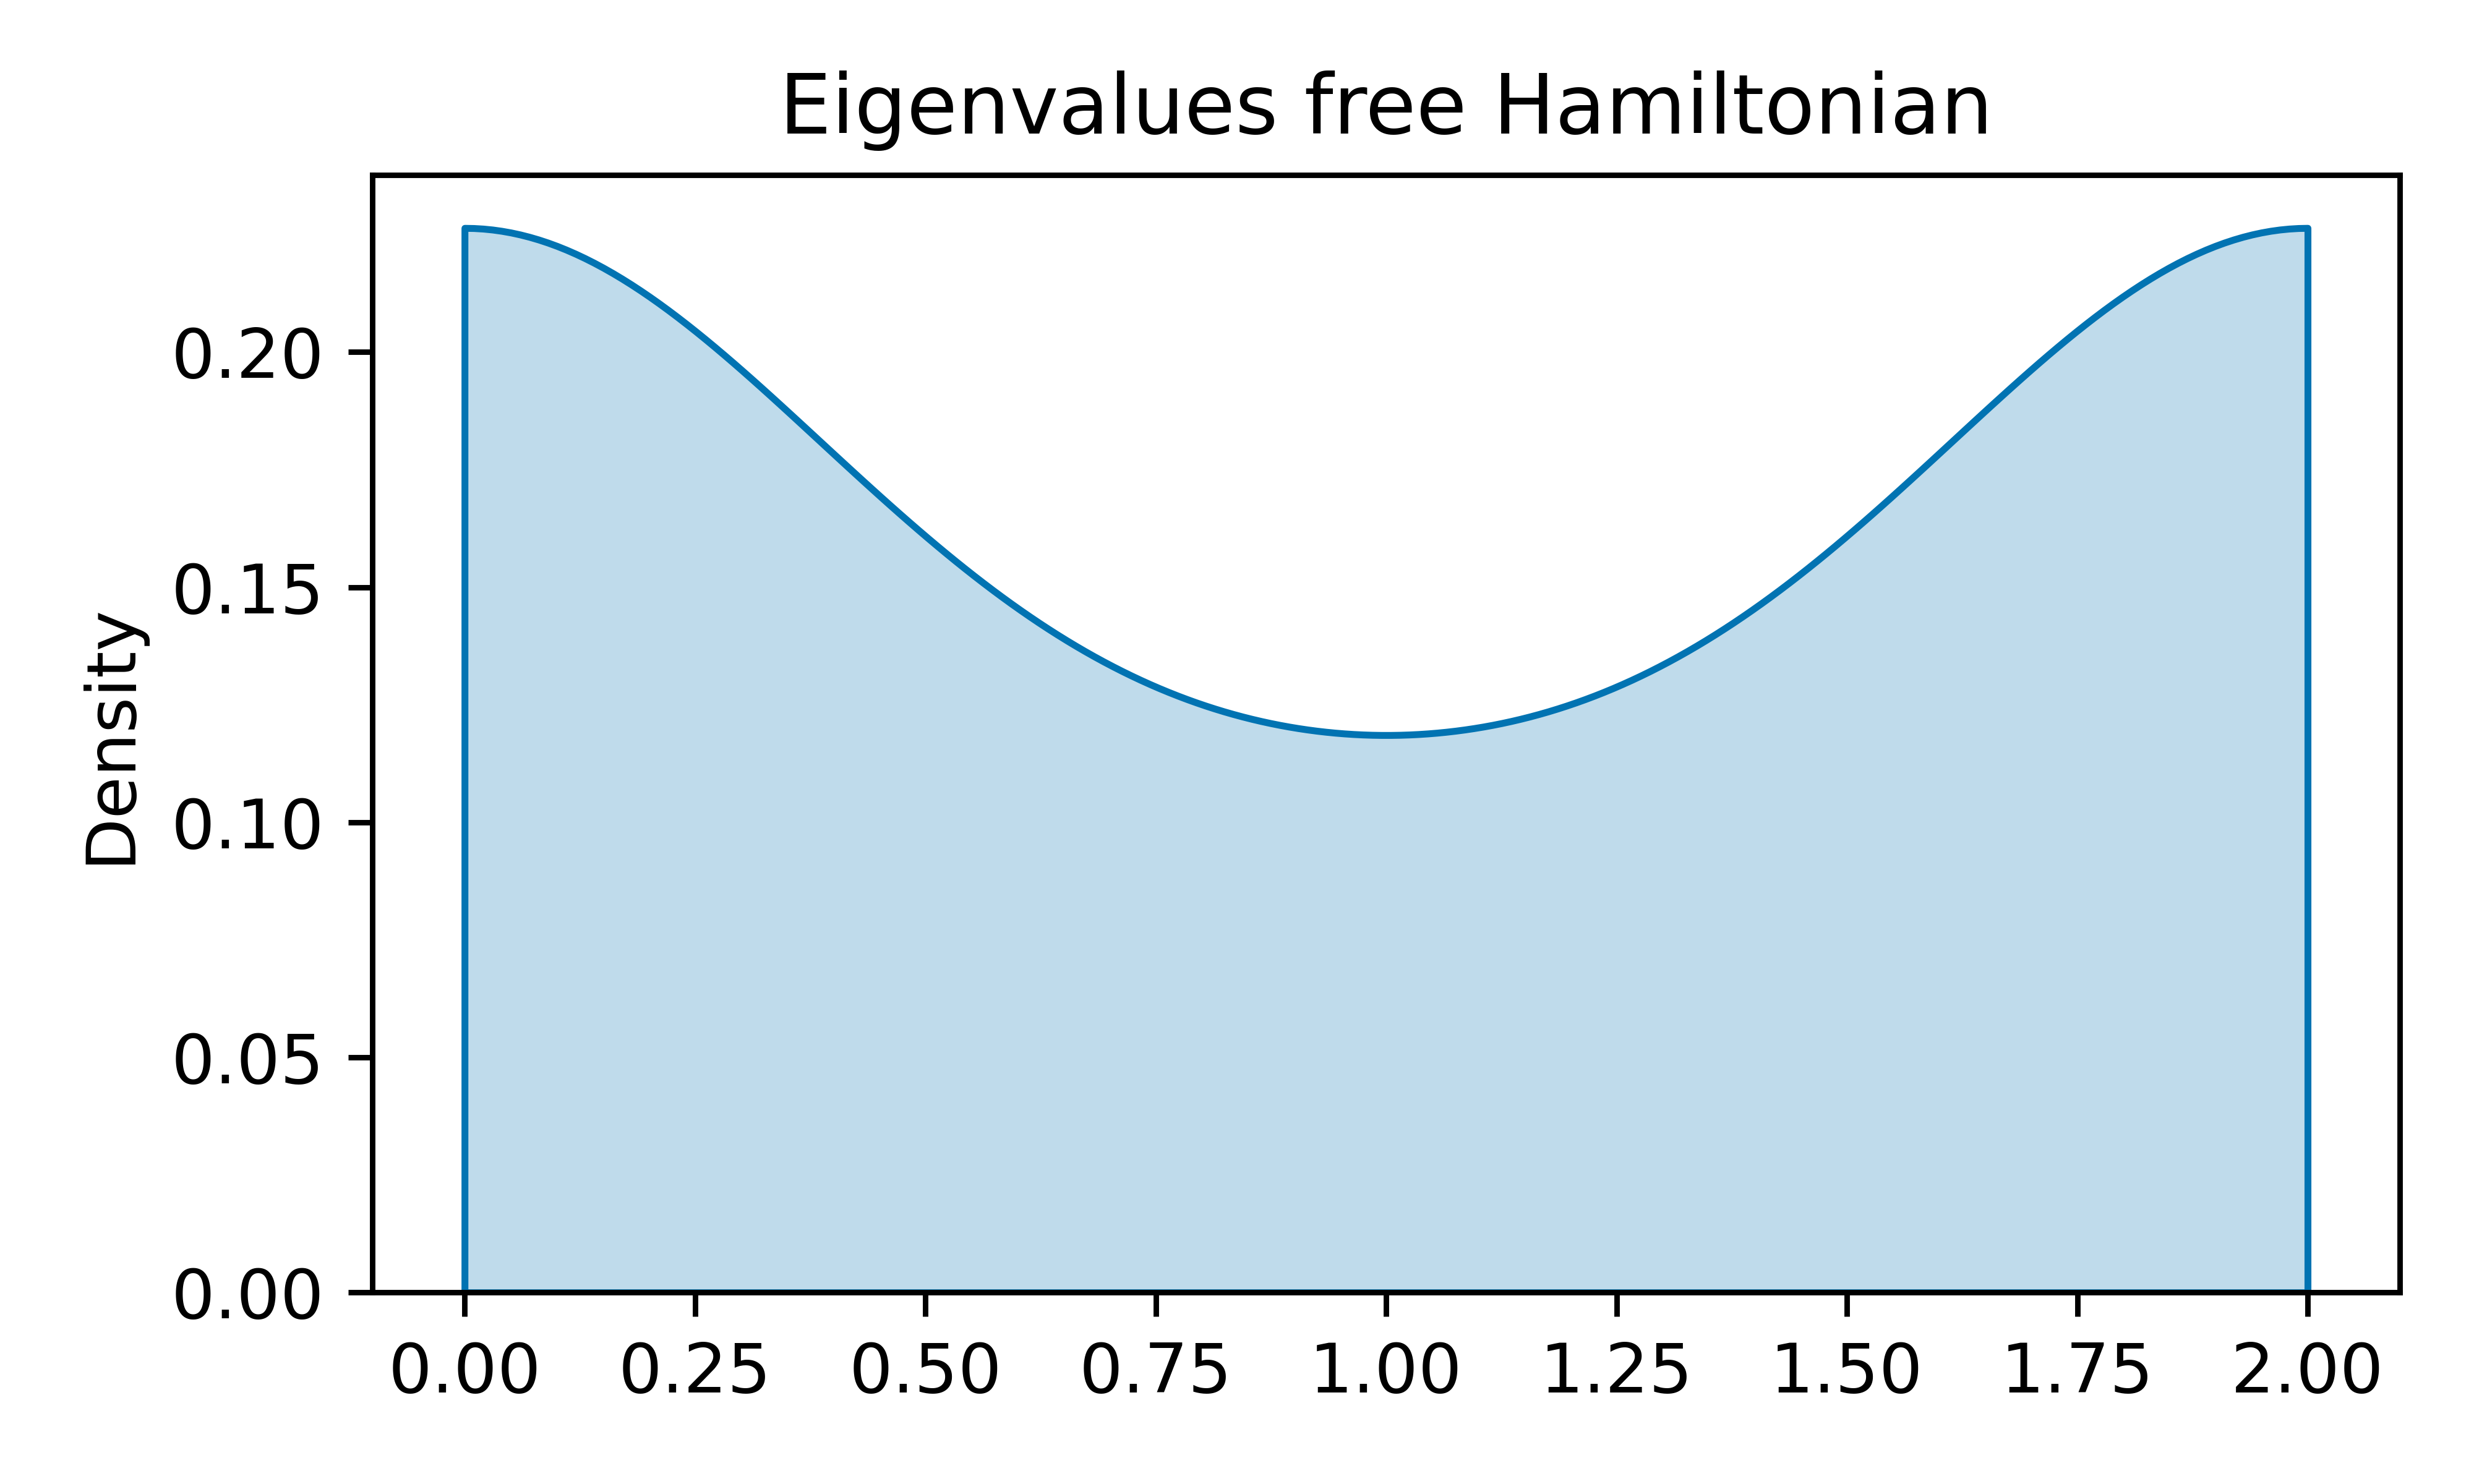
\includegraphics[scale=0.9]{kde_nonperturbed_L=1000.png}
   \caption{Kernel density estimation (KDE) plot of the spectrum of the free Hamiltonian, with $L = 1000$ and $\Delta x = 1$.}
   \label{fig:free_hamiltonian}
\end{figure}

Now, in order to validate the PIB and the SGB for this operator, first we need to take an uneven section. In fact, given the simplicity of $H_N$ and the periodic boundary conditions, we can choose any combination of $r, \lambda$ and $x$, and the singular value $\varepsilon_{r, \lambda, x}$ will still be independent of $x$, that is, it will be equal to the infimum $\varepsilon_{r, \lambda}$. For instance, let $r \in \{ 50, 100, 150, 200, 250 \}$, $\lambda \in \{ -0.1, 0.5, 1.2, 1.7, 2.3 \}$, and $x = 500$, then an uneven section will look like so

\[
    (H_N - \lambda I) = \begin{pmatrix}
        1 - \lambda & -\frac{1}{2} & & & & \cdots & & & & & & & -\frac{1}{2} \\
        -\frac{1}{2} & 1 - \lambda & & & & & & & & & & & \\
        & & \ddots & & & & & & & & & & \\
        & & & 1 - \lambda & \tikzmark{left}{$-\frac{1}{2}$} & & & & & & & & \\
        & & & -\frac{1}{2} & 1 - \lambda & -\frac{1}{2} & & & & & & & \\
        \vdots & & & & -\frac{1}{2} & 1 - \lambda & -\frac{1}{2} & & & & & & \vdots \\
        & & & & & \ddots & \ddots & \ddots & & & & & \\
        & & & & & & -\frac{1}{2} & 1 - \lambda & -\frac{1}{2} & & & & \\
        & & & & & & & \tikzmark{right}{$-\frac{1}{2}$} & 1 - \lambda & & & & \\
        & & & & & & & & & & \ddots & & \\
        & & & & & & & & & & & 1 - \lambda & -\frac{1}{2} \\
        -\frac{1}{2} & & & & & \cdots & & & & & & -\frac{1}{2} & 1 - \lambda
    \end{pmatrix}
    \Highlight[uneven_section]
    \tikz[overlay,remember picture] {
        \node[above of=uneven_section, xshift=45pt, yshift=9pt] {$Q_{r, \lambda, x}$};
    }
\]

And we get the following results:
\vspace{0.5cm}

\setlength{\tabcolsep}{8pt} % Default value: 6pt
\renewcommand{\arraystretch}{1.2} % Default value: 1

\begingroup
\begin{center}
    \begin{tabular}{ |c||c|c|c| }
        \hline
        \multicolumn{4}{|c|}{Upper and Lower Bounds on $\rho_H(\lambda)$} \\
        \hline
        $\left( r, \lambda \right)$ & $d\left(\lambda, \sigma(H)\right)$ & PIB (Upper bound) & SGB (Lower bound) \\
        \hline
        $(50, -0.1)$ & 0.100000 & 0.100507 & -0.031493 \\
        $(100, -0.1)$ & 0.100000 & 0.100125 & 0.034125 \\
        $(150, -0.1)$ & 0.100000 & 0.100055 & 0.056055 \\
        $(200, -0.1)$ & 0.100000 & 0.100031 & 0.067031 \\
        $(250, -0.1)$ & 0.100000 & 0.100020 & 0.073620 \\
        \hline
        $(50, 0.5)$ & 0.000906 & 0.026657 & -0.033343 \\
        $(100, 0.5)$ & 0.000906 & 0.013402 & -0.016598 \\
        $(150, 0.5)$ & 0.000906 & 0.008979 & -0.011021 \\
        $(200, 0.5)$ & 0.000906 & 0.006768 & -0.008232 \\
        $(250, 0.5)$ & 0.000906 & 0.005409 & -0.006591 \\
        \hline
        $(50, 1.2)$ & 0.002025 & 0.029876 & -0.030124 \\
        $(100, 1.2)$ & 0.002025 & 0.015225 & -0.014775 \\
        $(150, 1.2)$ & 0.002025 & 0.010161 & -0.009839 \\
        $(200, 1.2)$ & 0.002025 & 0.007644 & -0.007356 \\
        $(250, 1.2)$ & 0.002025 & 0.006125 & -0.005875 \\
        \hline
        $(50, 1.7)$ & 0.000978 & 0.021814 & -0.062186 \\
        $(100, 1.7)$ & 0.000978 & 0.011073 & -0.030927 \\
        $(150, 1.7)$ & 0.000978 & 0.007394 & -0.020606 \\
        $(200, 1.7)$ & 0.000978 & 0.005568 & -0.015432 \\
        $(250, 1.7)$ & 0.000978 & 0.004465 & -0.012335 \\
        \hline
        $(50, 2.3)$ & 0.300005 & 0.300494 & 0.144494 \\
        $(100, 2.3)$ & 0.300005 & 0.300123 & 0.222123 \\
        $(150, 2.3)$ & 0.300005 & 0.300055 & 0.248055 \\
        $(200, 2.3)$ & 0.300005 & 0.300031 & 0.261031 \\
        $(250, 2.3)$ & 0.300005 & 0.300020 & 0.268820 \\
        \hline
    \end{tabular}
\end{center}
\endgroup

\vspace{0.5cm}
These data show that both the PIB and the SGB are valid bounds in the present case. Moreover, as the window size ($r$) increases, the PIB decreases and the SGB increases. The reason for this is that a larger window captures more of the support of the eigenvector of $H_N$ corresponding to the eigenvalue closest to our chosen $\lambda$, and thus, the SVD can produce a better approximation to both the eigenvector and the eigenvalue. Another interesting pattern we can observe in the data is that values of $\lambda$ outside the spectrum range yield a PIB closer to $d\left(\lambda, \sigma(H)\right)$, likely due to the higher localization of edge states.

\newpage

\section{Conclusion and Future Work}

In this work we checked the validity of the pseudospectral inclusion bound and the spectral gap bound against the Hamiltonian describing the behavior of a free particle in one dimension. Additionally, we ran a sensitivity test on two of the variables of an uneven section, namely, $r$ and $\lambda$, which then enabled us to understand their effect on the calculation of the bounds.

Furthermore, we developed a computer program capable of computing the PIB and the SGB for any Hamiltonian represented by a finite matrix, thus making it possible for us to study a great variety of quantum systems.

Future work should focus on validating the bounds against different Hamiltonians, e.g., random Hamiltonians, Hamiltonians emerging from quasicrystal systems, etc., and developing software capable of proving spectral gaps of infinite-volume one-body operators.

\newpage

\printbibliography

\end{document}
